\subsection{Parameters identification results}
\label{subsec:parameters_identification_results}

Once the previously explained procedure has been applied to all the natural frequencies of the system (consider for each one, every experimental FRFs at our disposal), we can reassemble the identified parameters so to compute the numerical FRFs of the system based on Equation \ref{eq:FRF_approximation}.

In the following figures, the result obtained considering the FRF relative to an input in $x_k = 1.0m$ and an output in $y_j = 0.6m$ is shown.

\begin{figure}[H]
    \centering
    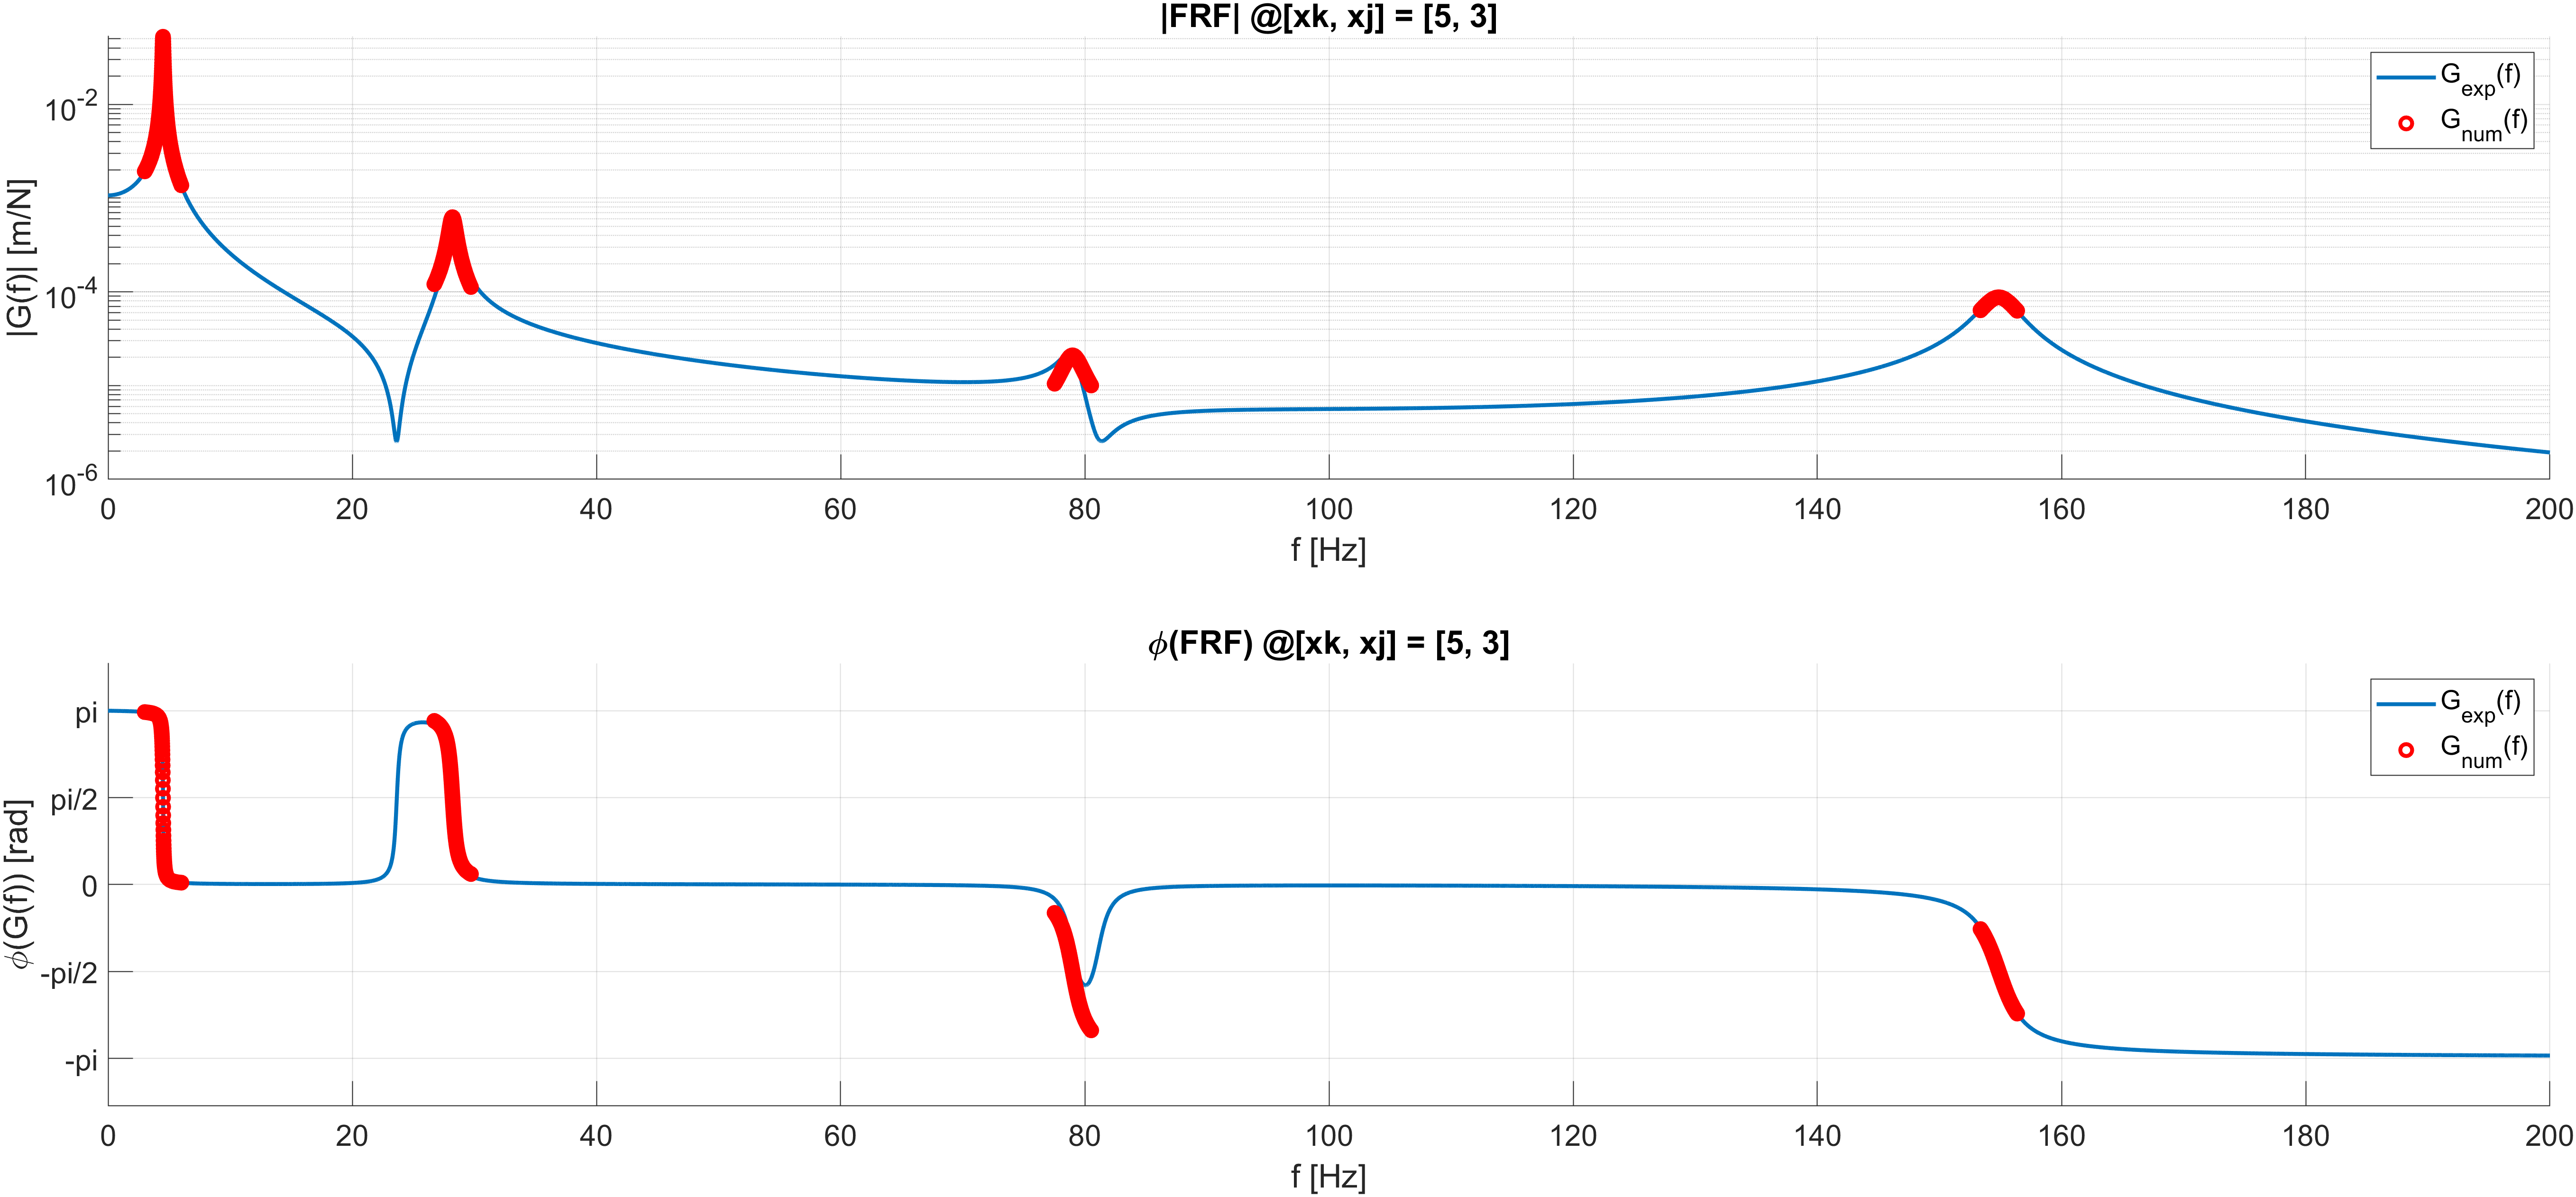
\includegraphics[width=\textwidth]{img/MATLAB/Part_A/Comparison_FRF_couple_3_5.png}
    \caption{FRF identification for $x_k = 1.0m$ and $y_j = 0.6m$}
    \label{fig:FRF_identification}
\end{figure}

\begin{figure}[H]
    \begin{minipage}[b]{0.45\textwidth}
        \centering
        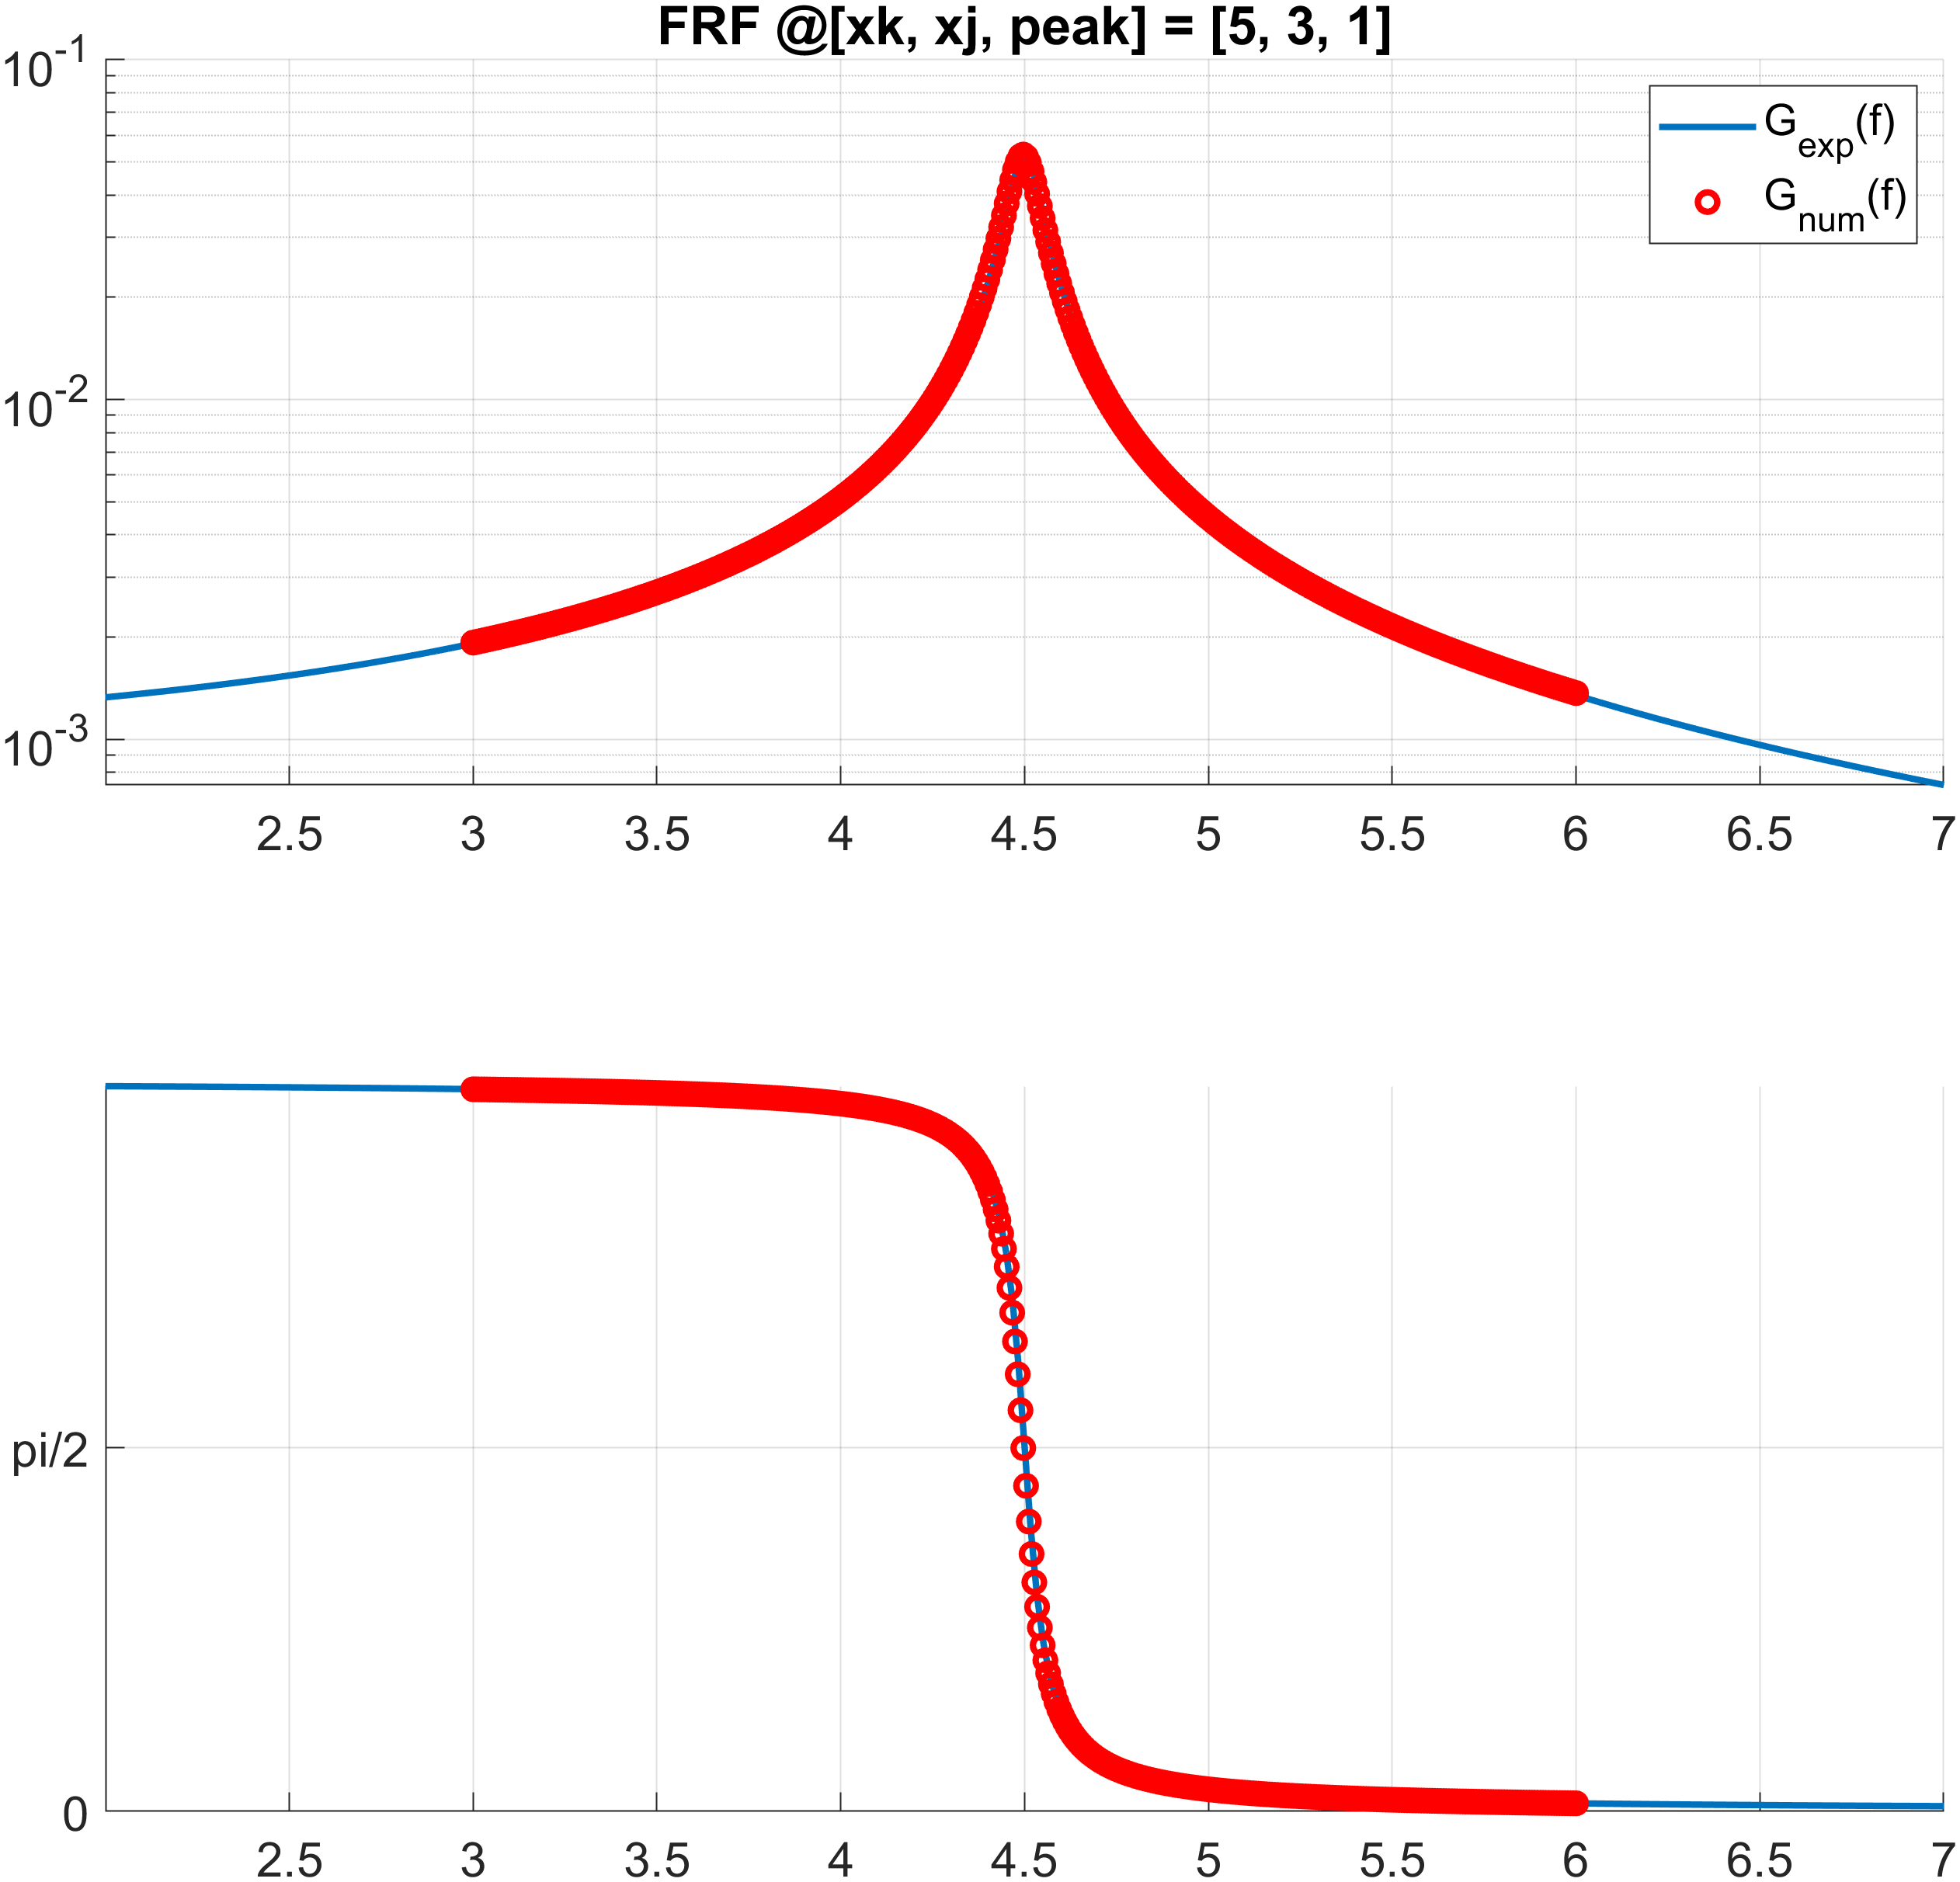
\includegraphics[width=\textwidth]{img/MATLAB/Part_A/Comparison_FRF_couple_3_5_zoom_peak_01.png}
    \end{minipage}
    \hfill
    \begin{minipage}[b]{0.45\textwidth}
        \centering
        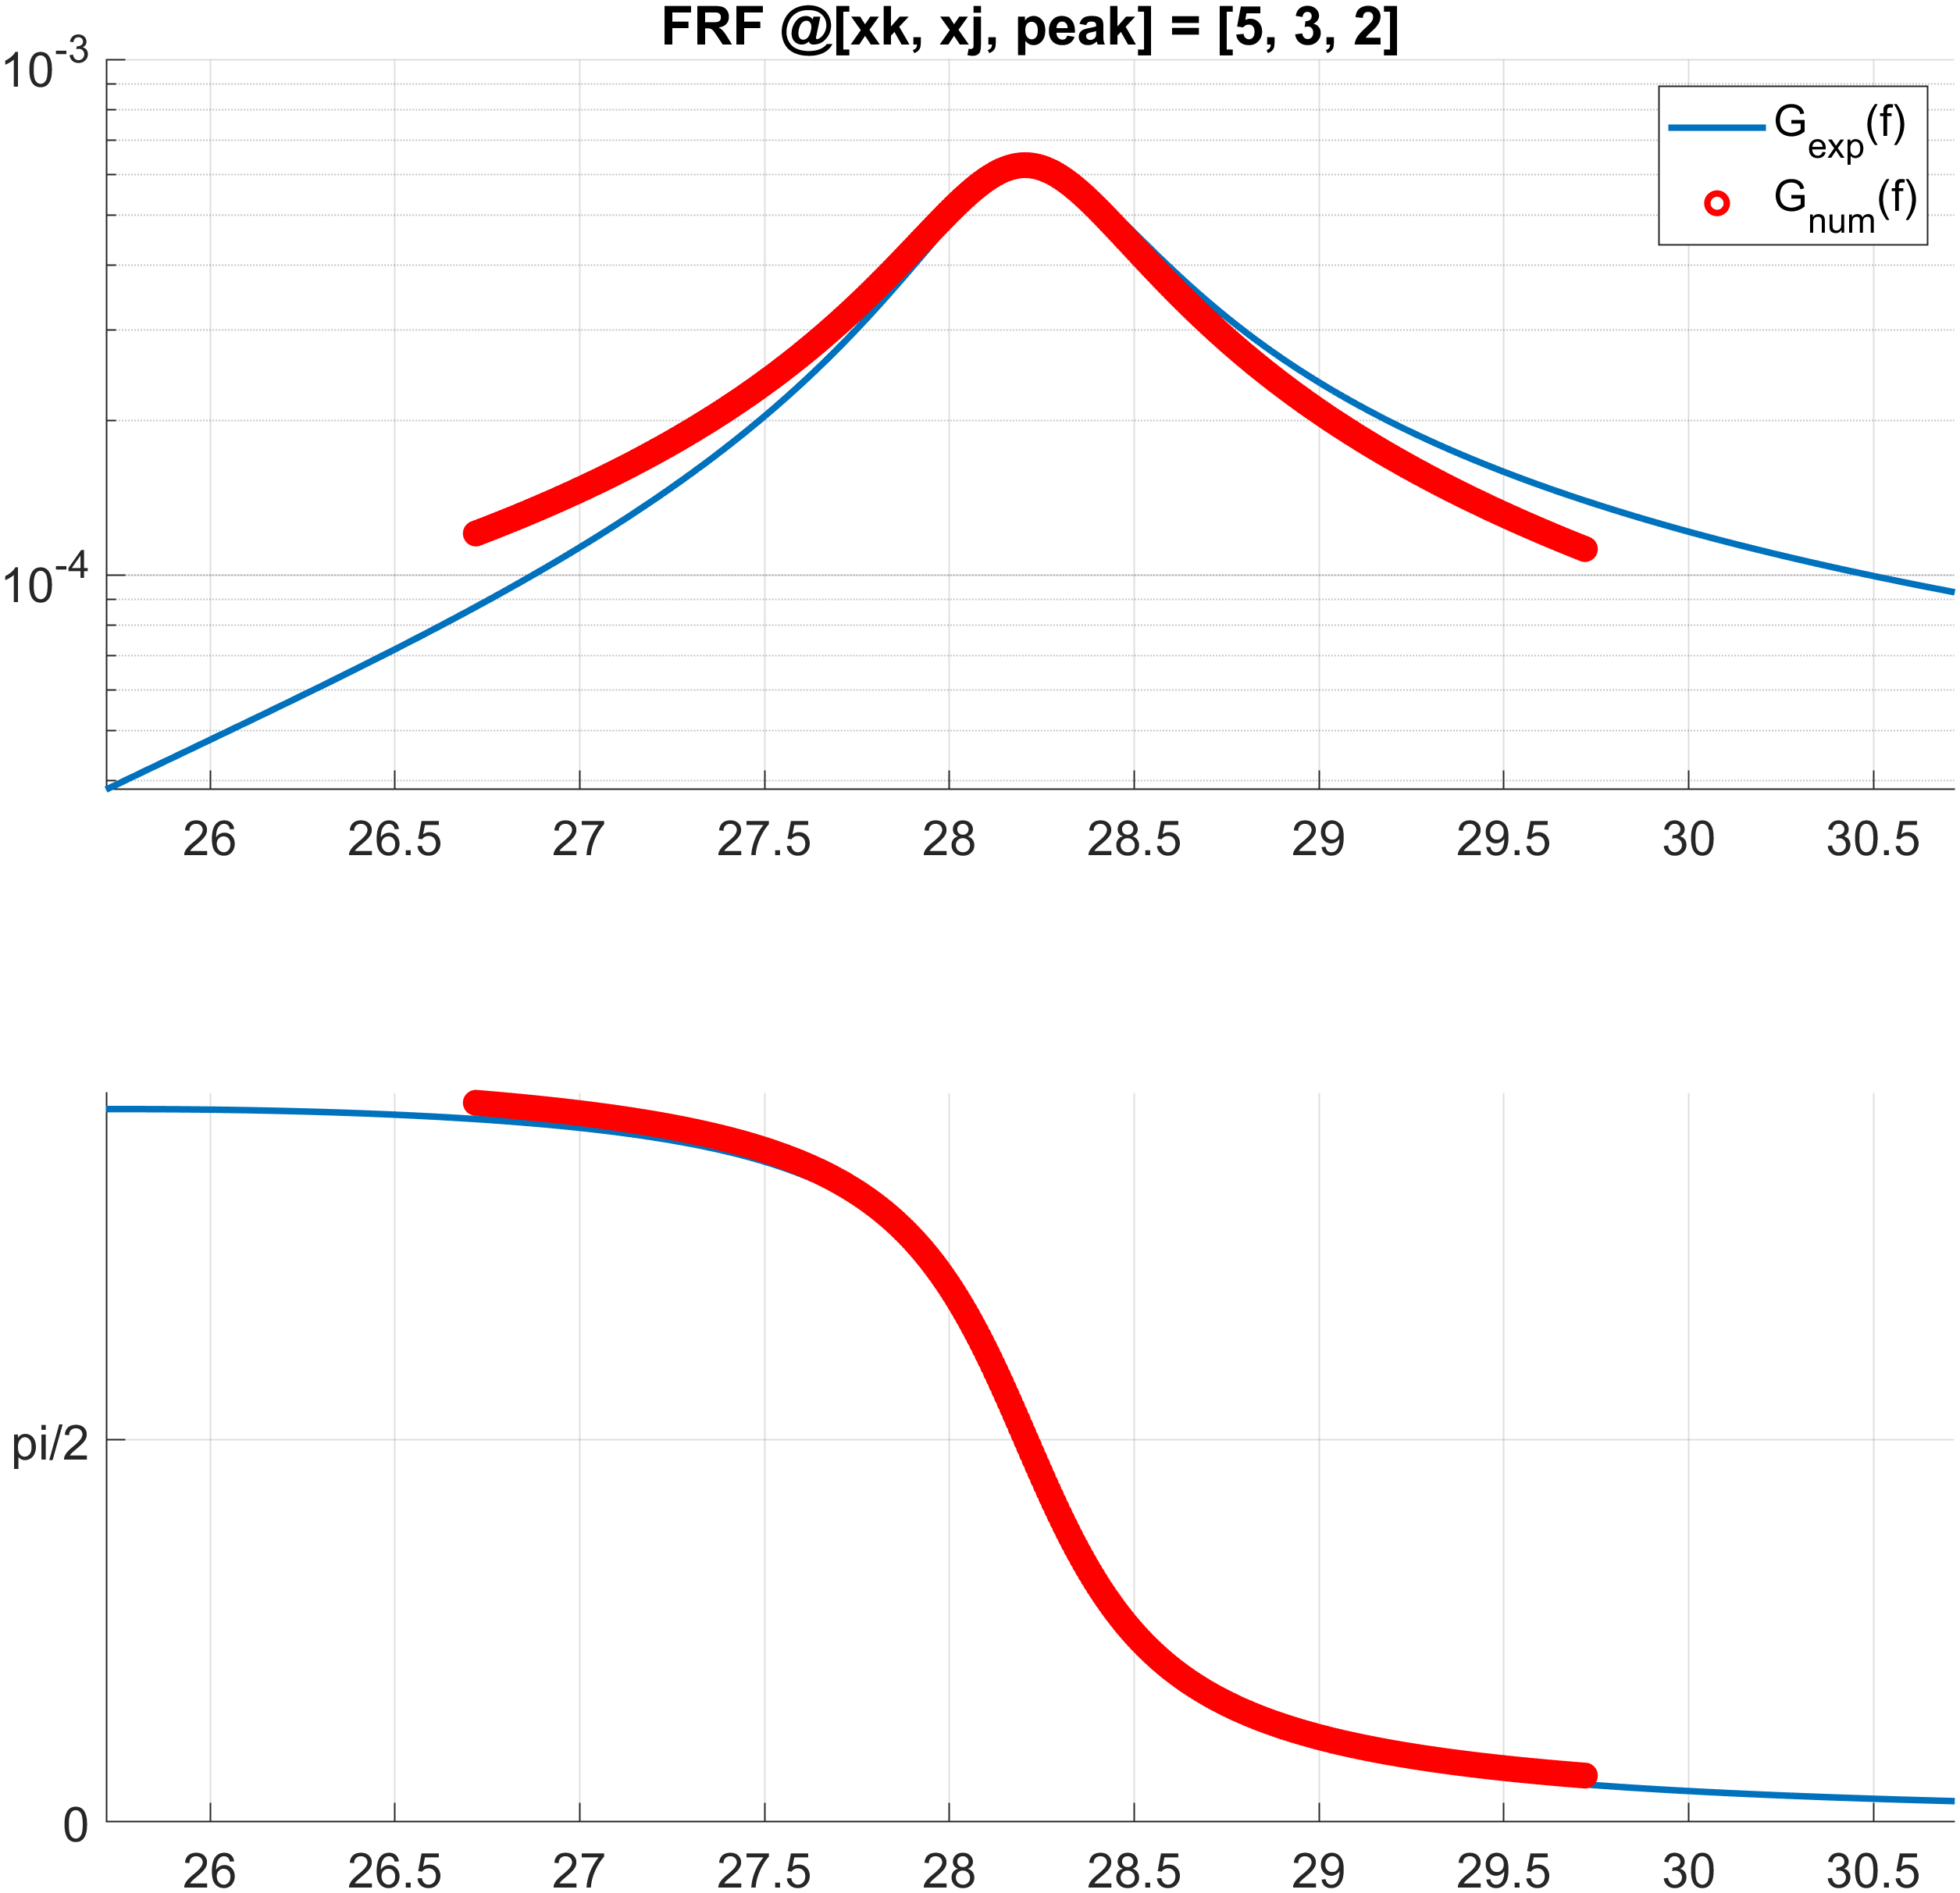
\includegraphics[width=\textwidth]{img/MATLAB/Part_A/Comparison_FRF_couple_3_5_zoom_peak_02.png}
    \end{minipage}
    \begin{minipage}[b]{0.45\textwidth}
        \centering
        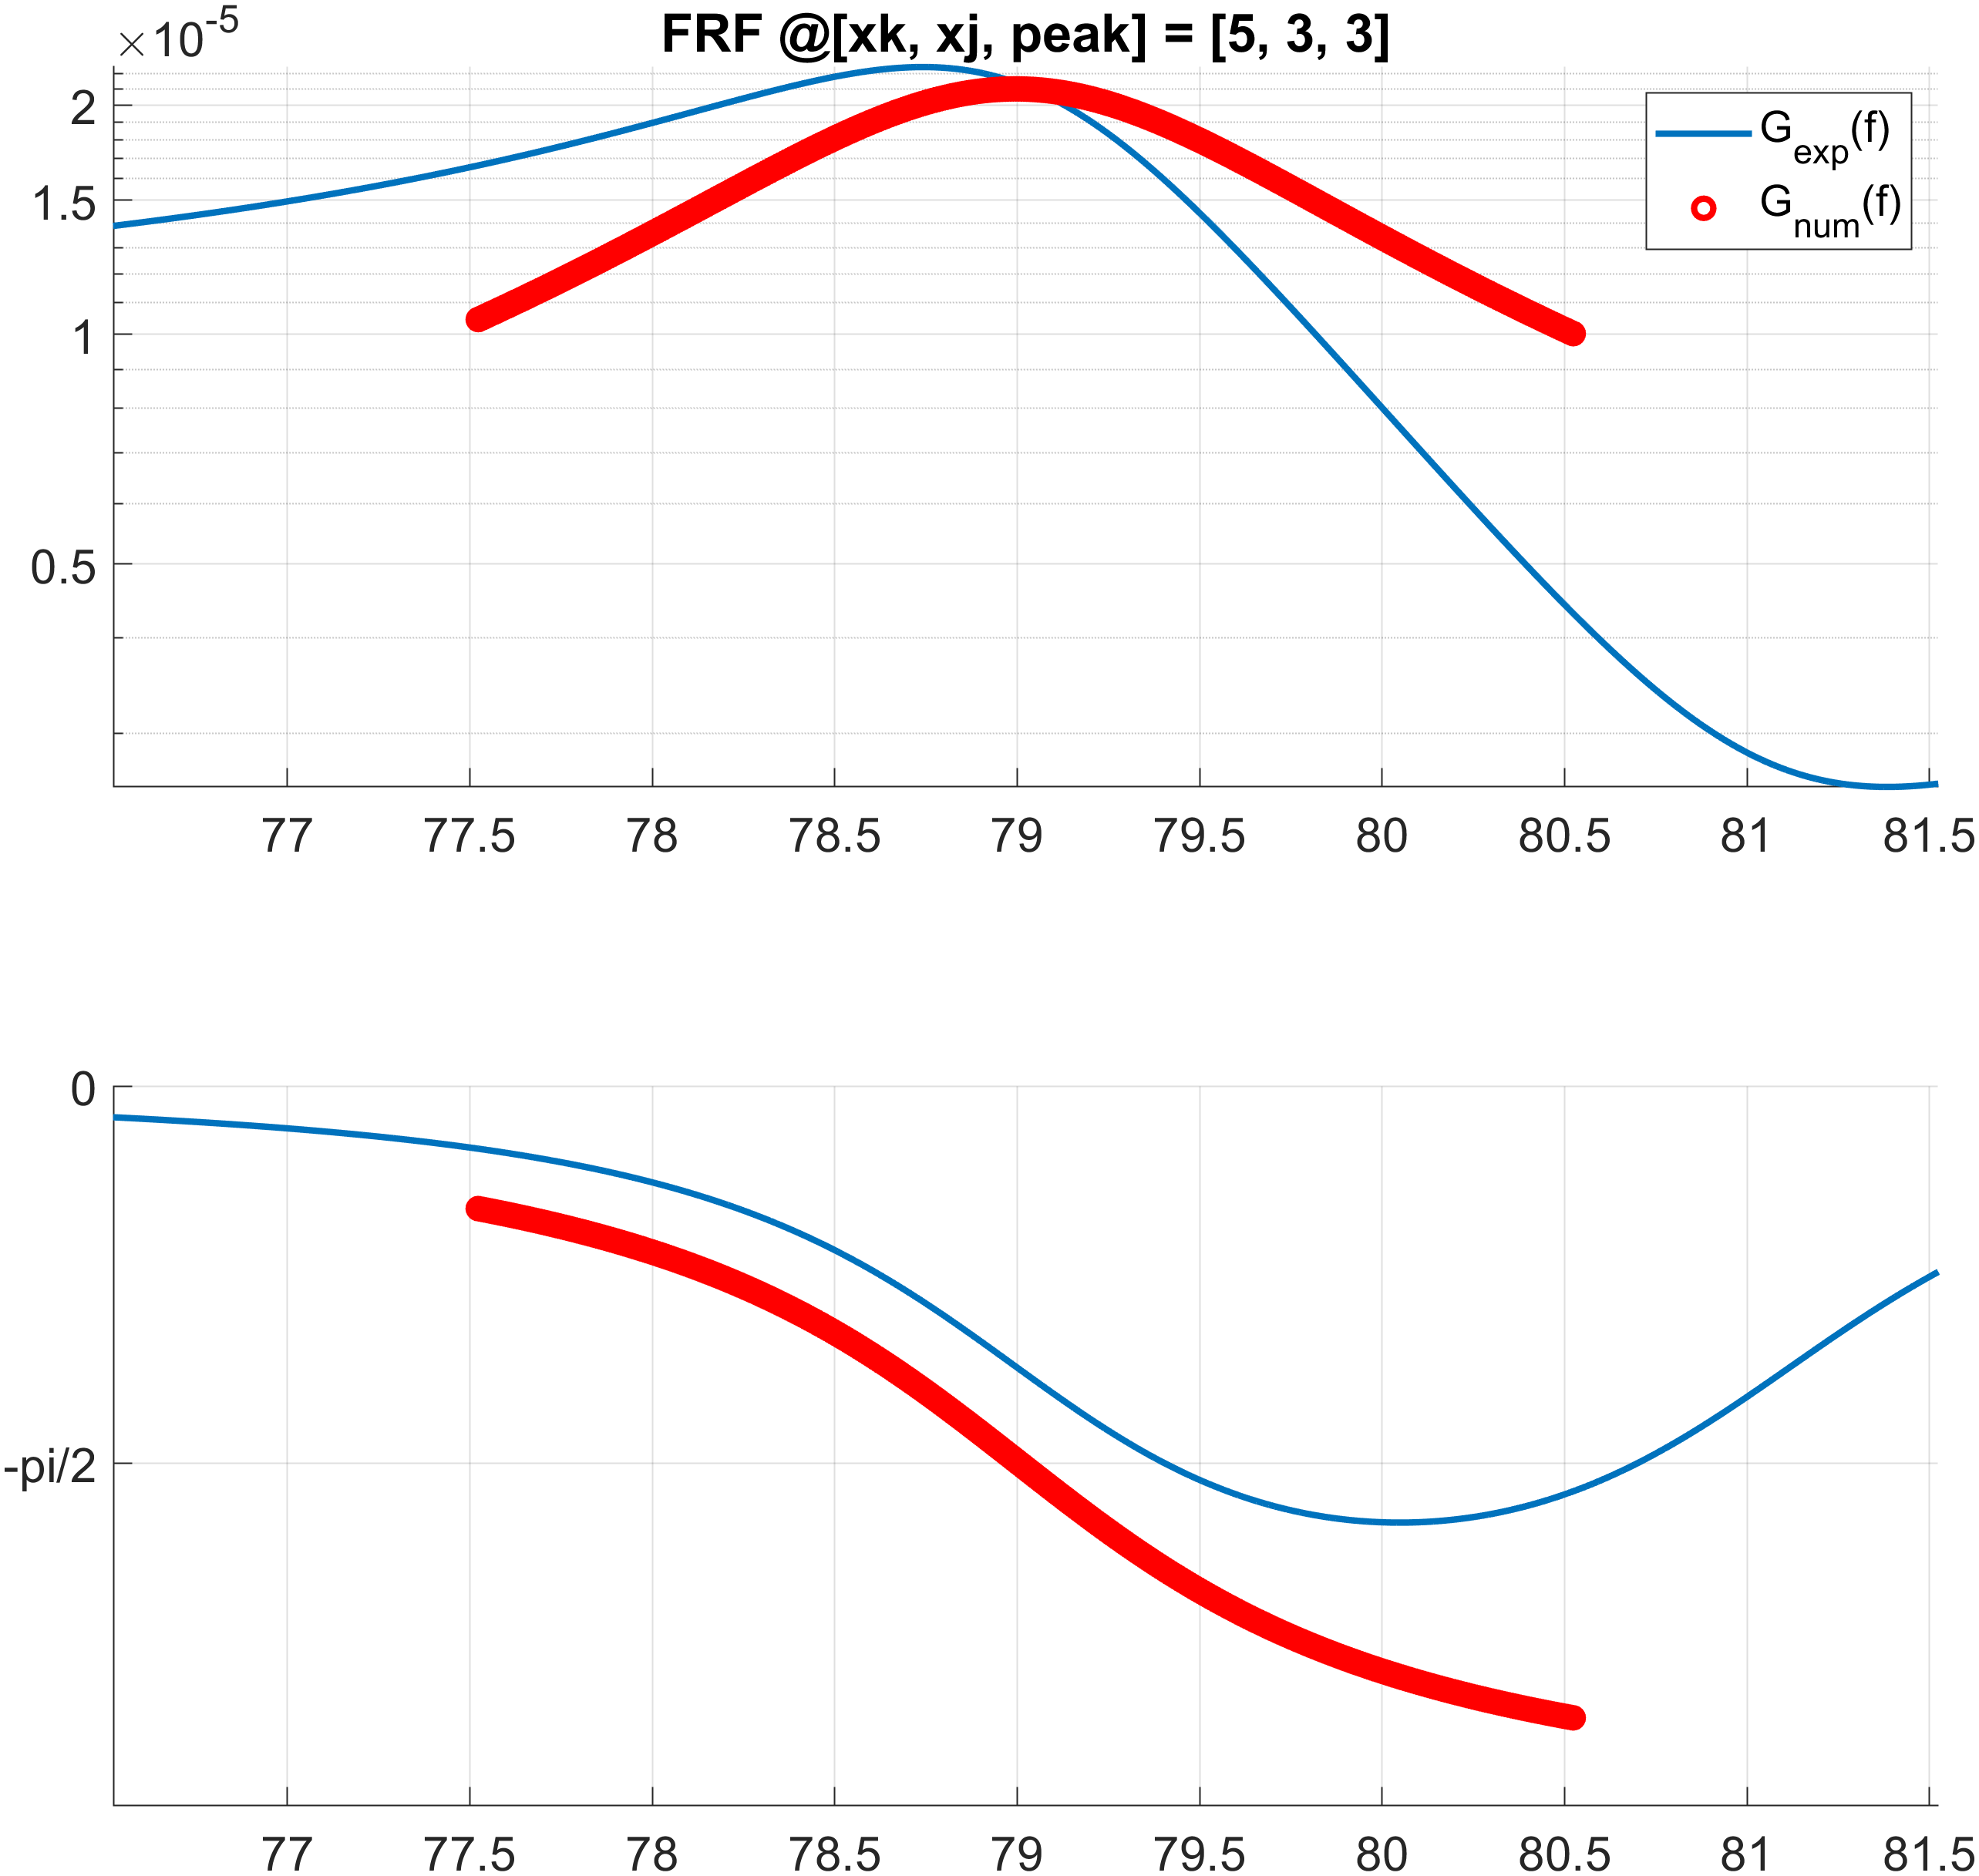
\includegraphics[width=\textwidth]{img/MATLAB/Part_A/Comparison_FRF_couple_3_5_zoom_peak_03.png}
    \end{minipage}
    \hfill
    \begin{minipage}[b]{0.45\textwidth}
        \centering
        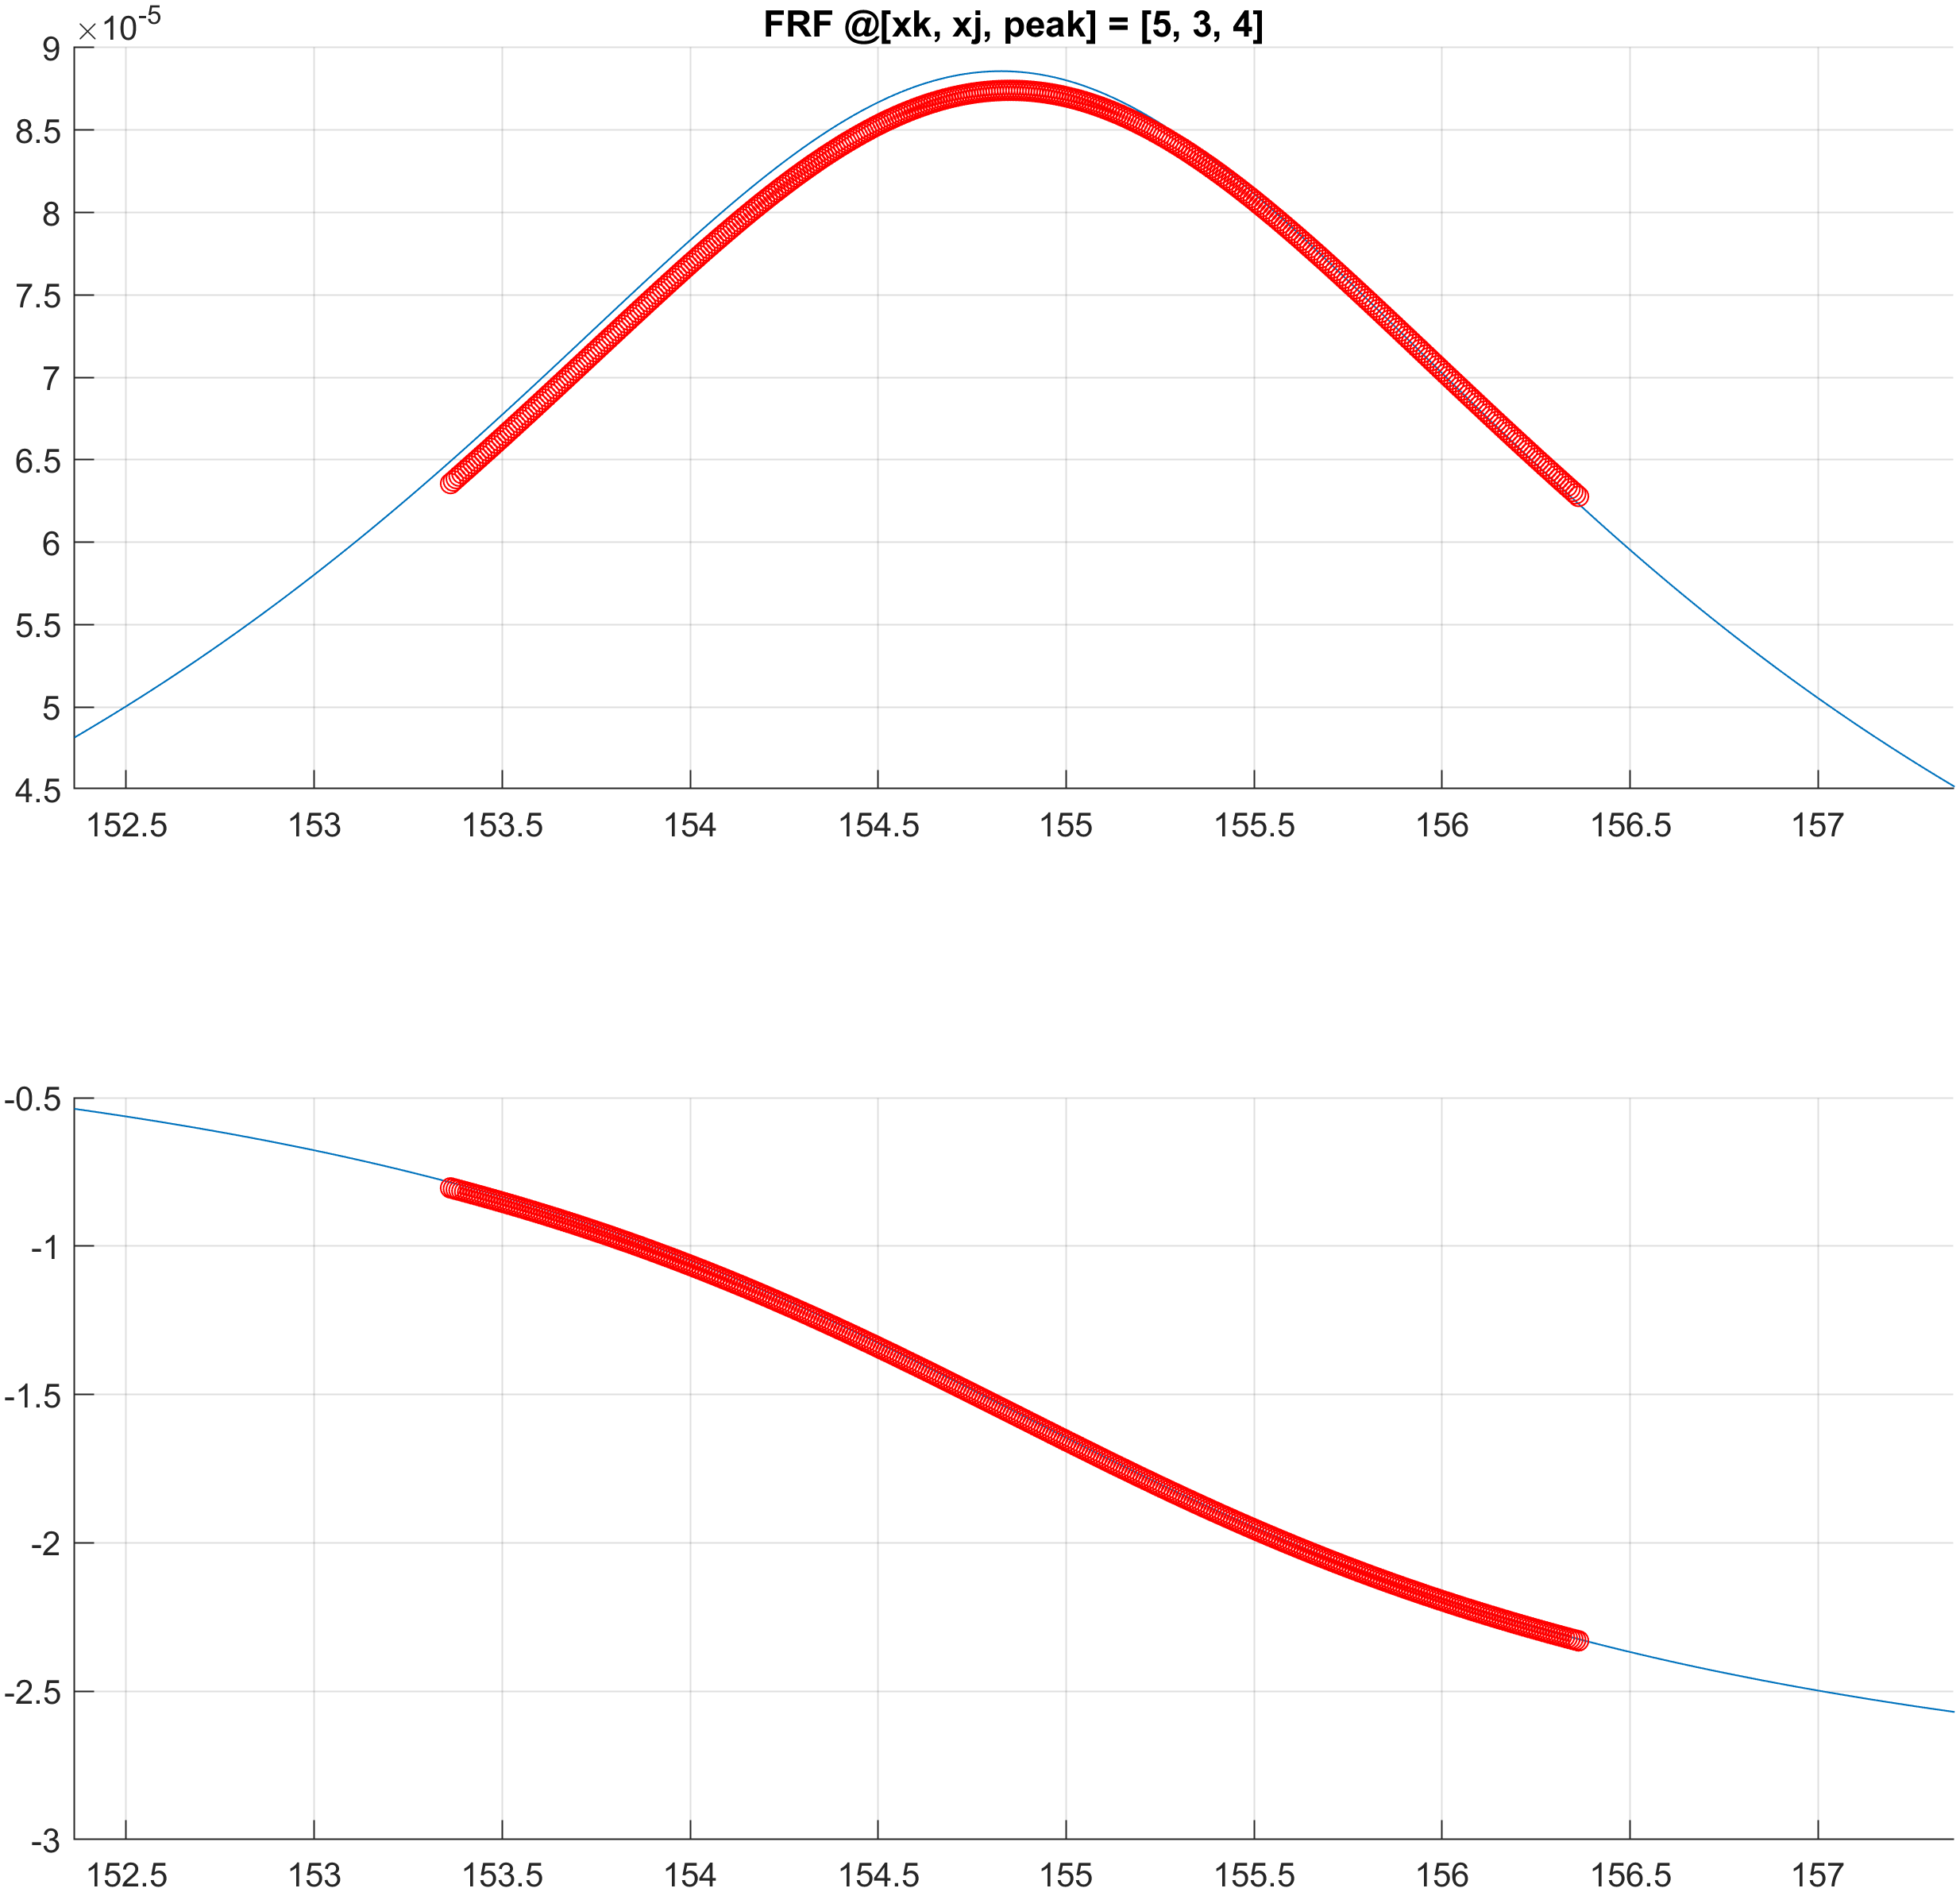
\includegraphics[width=\textwidth]{img/MATLAB/Part_A/Comparison_FRF_couple_3_5_zoom_peak_04.png}
    \end{minipage}
    \caption{Zoom over the peaks of the FRF identification for $x_k = 1.0m$ and $y_j = 0.6m$}
    \label{fig:FRF_identification_zoom}
\end{figure}
